
%{{第三十三回}}{第三十三回}}

\chapter{手足耽耽小动唇舌 不肖种种大承笞挞}\label{part0037_split_000.htmlux5cux23calibre_pb_0}

{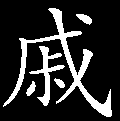
\includegraphics[width=3mm]{../Images/00005}富贵公子,侯王应袭,容易在红粉场中作罪。风流情性,诗赋文词,偏只为莺花路间留滞。笑嘻嘻,哭啼啼,总是一般情事。}

却说王夫人唤他母亲上来,拿几件簪环当面赏与,又吩咐请几众僧人念经超度。他母亲磕头谢了出去。

原来宝玉会过雨村回来听见了,便知金钏儿含羞赌气自尽,心中早又五内摧伤,进来被王夫人数落教训,也无可回说。见宝钗进来,方得便出来,茫然不知何往,背着手,低头一面感叹,一面慢慢的走着,信步来至厅上。刚转过屏门,不想对面来了一人正往里走,可巧儿撞了个满怀。只听那人喝了一声``站住!''宝玉唬了一跳,抬头一看,不是别人,却是他父亲,不觉的倒抽了一口气,只得垂手一旁站了。贾政道:``好端端的,你垂头丧气嗐些什么?方才雨村来了要见你,叫你那半天你才出来;既出来了,全无一点慷慨挥洒谈吐,仍是葳葳蕤蕤。我看你脸上一团思欲愁闷气色,这会子又咳声叹气。你那些还不足,还不自在?无故这样,却是为何?''宝玉素日虽是口角伶俐,只是此时一心总为金钏儿感伤,恨不得此时也身亡命殒,{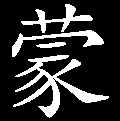
\includegraphics[width=3mm]{../Images/00006}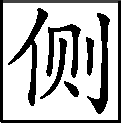
\includegraphics[width=3mm]{../Images/00011}\footnotesize \kaishu 真有此情,真有此理。}跟了金钏儿去。如今见了他父亲说这些话,究竟不曾听见,只是怔呵呵的站着。

贾政见他惶悚,应对不似往日,原本无气的,这一来倒生了三分气。方欲说话,忽有回事人来回:``忠顺亲王府里有人来,要见老爷。''贾政听了,心下疑惑,暗暗思忖道:``素日并不和忠顺府来往,为什么今日打发人来?''一面想,一面令``快请'',急走出来看时,却是忠顺府长史官,忙接进厅上坐了献茶。

未及叙谈,那长史官先就说道:``下官此来,并非擅造潭府,皆因奉王命而来,有一件事相求。看王爷面上,敢烦老大人作主,不但王爷知情,且连下官辈亦感谢不尽。''贾政听了这话,抓不住头脑,忙陪笑起身问道:``大人既奉王命而来,不知有何见谕,望大人宣明,学生好遵谕承办。''那长史官便冷笑道:``也不必承办,只用大人一句话就完了。我们府里有一个做小旦的琪官,一向好好在府里,如今竟三五日不见回去,各处去找,又摸不着他的道路,因此各处访察。这一城内,十停人倒有八停人都说,他近日和衔玉的那位令郎相与甚厚。下官辈等听了,尊府不比别家,可以擅入索取,因此启明王爷。王爷亦云:`若是别的戏子呢,一百个也罢了;只是这琪官随机应答,谨慎老诚,甚合我老人家的心,竟断断少不得此人。'故此求老大人转谕令郎,请将琪官放回,一则可慰王爷谆谆奉恳,二则下官辈也可免操劳求觅之苦。''{
}\href{../Text/part0037_split_000.html\#lnkback_1_a}{\textsuperscript{①}}说毕,忙打一躬。

贾政听了这话,又惊又气,即命唤宝玉来。宝玉也不知是何原故,忙赶来时,贾政便问:``该死的奴才!你在家不读书也罢了,怎么又做出这些无法无天的事来!那琪官现是忠顺王爷驾前承奉的人,你是何等草芥,无故引逗他出来,如今祸及于我。''宝玉听了唬了一跳,忙回道:``实在不知此事。究竟连`琪官'两个字不知为何物,岂更又加`引逗'二字!''说着便哭了。

贾政未及开言,只见那长史官冷笑道:``公子也不必掩饰。或隐藏在家,或知其下落,早说了出来,我们也少受些辛苦,岂不念公子之德?''宝玉连说不知,``恐是讹传,也未见得。''那长史官冷笑道:``现有据证,何必还赖?必定当着老大人说了出来,公子岂不吃亏?既云不知此人,那红汗巾子怎么到了公子腰里?''宝玉听了这话,不觉轰去魂魄,目瞪口呆,心下自思:``这话他如何得知!他既连这样机密事都知道了,大约别的瞒他不过,不如打发他去了,免的再说出别的事来。''因说道:``大人既知他的底细,如何连他置买房舍这样大事倒不晓得了?听得说他如今在东郊离城二十里有个什么紫檀堡,他在那里置了几亩田地几间房舍。想是在那里也未可知。''那长史官听了,笑道:``这样说,一定是在那里。我且去找一回,若有了便罢,若没有,还要来请教。''{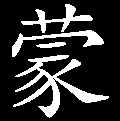
\includegraphics[width=3mm]{../Images/00006}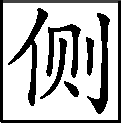
\includegraphics[width=3mm]{../Images/00011}\footnotesize \kaishu 宝玉其人,爱之有馀,岂可挞者?用此等文章逼之,能不使人肝胆愤烈,以成下文之严酷耶?}说着,便忙忙的走了。

贾政此时气的目瞪口歪,一面送那长史官,一面回头命宝玉``不许动!回来有话问你!''一直送那官员去了。才回身,忽见贾环带着几个小厮一阵乱跑。贾政喝令小厮``快打,快打!''贾环见了他父亲,唬的骨软筋酥,忙低头站住。贾政便问:``你跑什么?带着你的那些人都不管你,不知往那里逛去,由你野马一般!''喝令叫跟上学的人来。贾环见他父亲盛怒,便乘机说道:``方才原不曾跑,只因从那井边一过,那井里淹死了一个丫头,我看见人头这样大,身子这样粗,泡的实在可怕,所以才赶着跑了过来。''贾政听了惊疑,问道:``好端端的,谁去跳井?我家从无这样事情,自祖宗以来,皆是宽柔以待下人。------大约我近年于家务疏懒,自然执事人操克夺之权,致使生出这暴殄轻生的祸患。若外人知道,祖宗颜面何在!''喝令快叫贾琏、赖大{{(兴)}}来\href{../Text/part0037_split_000.html\#lnkback_2_a}{\textsuperscript{②}}。

小厮们答应了一声,方欲叫去,贾环忙上前拉住贾政的袍襟,贴膝跪下道:``父亲不用生气。此事除太太房里的人,别人一点也不知道。我听见我母亲说\ldots{}\ldots{}''说到这里,便回头四顾一看。{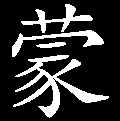
\includegraphics[width=3mm]{../Images/00006}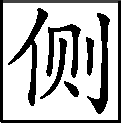
\includegraphics[width=3mm]{../Images/00011}\footnotesize \kaishu 如画。}贾政知意,将眼一看众小厮,小厮们明白,都往两边后面退去。贾环便悄悄说道:``我母亲告诉我说,宝玉哥哥前日在太太屋里,拉着太太的丫头金钏儿强奸不遂,{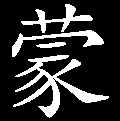
\includegraphics[width=3mm]{../Images/00006}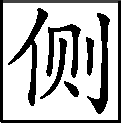
\includegraphics[width=3mm]{../Images/00011}\footnotesize \kaishu 再逼下文,有不得不尽情苦打之势。}打了一顿。那金钏儿便赌气投井死了。''话未说完,把个贾政气的面如金纸,大喝:``快拿宝玉来!''一面说,一面便往里边书房里去,喝令:``今日再有人劝我,我把这冠带家私一应交与他与宝玉过去!我免不得做个罪人,把这几根烦恼鬓毛剃去,寻个干净去处自了,也免得上辱先人下生逆子之罪。''{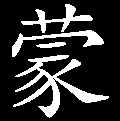
\includegraphics[width=3mm]{../Images/00006}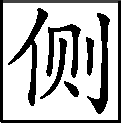
\includegraphics[width=3mm]{../Images/00011}\footnotesize \kaishu 一激再激,实文实事。}众门客仆从见贾政这个形景,便知又是为宝玉了,一个个都是啖指咬舌,连忙退出。那贾政喘吁吁直挺挺坐在椅子上,满面泪痕,{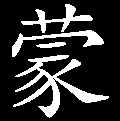
\includegraphics[width=3mm]{../Images/00006}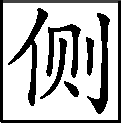
\includegraphics[width=3mm]{../Images/00011}\footnotesize \kaishu 为天下父母一哭。}一叠声``拿宝玉!拿大棍!拿索子捆上!把各门都关上!有人传信往里头去,立刻打死!''众小厮们只得齐声答应,有几个来找宝玉。

那宝玉听见贾政吩咐他``不许动'',早知多凶少吉,那里承望贾环又添了许多的话。正在厅上干转,怎得个人来往里头去捎信,偏生没个人,连茗烟也不知在那里。正盼望时,只见一个老姆姆出来。宝玉如得了珍宝,便赶上来拉他,说道:``快进去告诉:老爷要打我呢!快去,快去!要紧,要紧!''宝玉一则急了,说话不明白;二则老婆子偏生又聋,竟不曾听见是什么话,把``要紧''二字只听作``跳井''二字,便笑道:``跳井让他跳去,二爷怕什么?''宝玉见是个聋子,便着急道:``你出去叫我的小厮来罢。''那婆子道:``有什么不了的事?老早的完了。太太又赏了衣服,又赏了银子,怎么不了事的!''{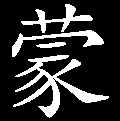
\includegraphics[width=3mm]{../Images/00006}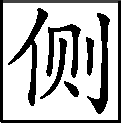
\includegraphics[width=3mm]{../Images/00011}\footnotesize \kaishu 写老婆子爱说无要紧的话,真如见其人,如闻其声。}

宝玉急的跺脚,正没抓寻处,只见贾政的小厮走来,逼着他出去了。贾政一见,眼都红紫了,也不暇问他在外流荡优伶,表赠私物,在家荒疏学业,淫辱母婢等语,{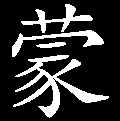
\includegraphics[width=3mm]{../Images/00006}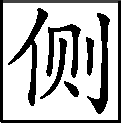
\includegraphics[width=3mm]{../Images/00011}\footnotesize \kaishu 了结得灵活。}只喝令:``堵起嘴来,着实打死!''小厮们不敢违拗,只得将宝玉按在凳上,举起大板打了十来下。贾政犹嫌打轻了,一脚踢开掌板的,自己夺过来,咬着牙狠命盖了三四十下。众门客见打的不祥了,忙上前夺劝。贾政那里肯听,说道:``你们问问他干的勾当可饶不可饶!素日皆是你们这些人把他酿坏了,到这步田地还来解劝。明日酿到他弑君杀父,你们才不劝不成!''

众人听这话不好听,知道气急了,忙又退出,只得觅人进去给信。王夫人不敢先回贾母,只得忙穿衣出来,也不顾有人没人,忙忙赶往书房中来,{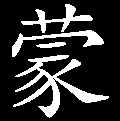
\includegraphics[width=3mm]{../Images/00006}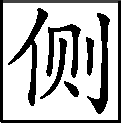
\includegraphics[width=3mm]{../Images/00011}\footnotesize \kaishu 为天下慈母一哭。}慌的众门客小厮等避之不及。王夫人一进房来,贾政更如火上浇油一般,那板子越发下去的又狠又快。按宝玉的两个小厮忙松了手走开,宝玉早已动弹不得了。贾政还欲打时,早被王夫人抱住板子。贾政道:``罢了,罢了!今日必定要气死我才罢!''王夫人哭道:``宝玉虽然该打,老爷也要自重。况且炎天暑日的,老太太身上也不大好,打死宝玉事小,倘或老太太一时不自在了,岂不事大!''{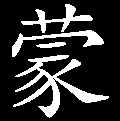
\includegraphics[width=3mm]{../Images/00006}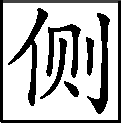
\includegraphics[width=3mm]{../Images/00011}\footnotesize \kaishu 父母之心,昊天罔极。贾政、王夫人易地则皆然。}贾政冷笑道:``倒休提这话。我养了这不肖的孽障,已经不孝;教训他一番,又有众人护持;不如趁今日一发勒死了,以绝将来之患!''说着,便要绳索来勒死。

王夫人连忙抱住哭道:``老爷虽然应当管教儿子,也要看夫妻分上。我如今已将五十岁的人,只有这个孽障,必定苦苦的以他为法,我也不敢深劝。今日越发要他死,岂不是有意绝我。既要勒死他,快拿绳子来先勒死我,再勒死他。我们娘儿们不敢含怨,到底在阴司里得个依靠。''{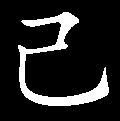
\includegraphics[width=3mm]{../Images/00003}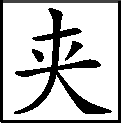
\includegraphics[width=3mm]{../Images/00012}\footnotesize \kaishu 未丧母者来细玩,既丧母者来痛哭。 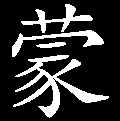
\includegraphics[width=3mm]{../Images/00006}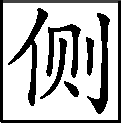
\includegraphics[width=3mm]{../Images/00011}\footnotesize \kaishu 使人读之,声哽咽而泪如雨下。}说毕,爬在宝玉身上大哭起来。贾政听了此话,不觉长叹一声,向椅上坐了,泪如雨下。王夫人抱着宝玉,只见他面白气弱,底下穿着一条绿纱小衣皆是血渍。禁不住解下汗巾看,由臀至胫,或青或紫,或整或破,竟无一点好处,不觉失声大哭起来,``苦命的儿吓!''因哭出``苦命儿''来,忽又想起贾珠来,便叫着贾珠哭道:``若有你活着,便死一百个我也不管了。''此时里面的人闻得王夫人出来,那李宫裁、王熙凤与迎春姊妹早已出来了。王夫人哭着贾珠的名字,{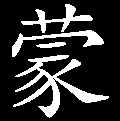
\includegraphics[width=3mm]{../Images/00006}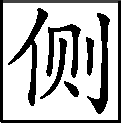
\includegraphics[width=3mm]{../Images/00011}\footnotesize \kaishu 慈母如画。}别人还可,惟有宫裁禁不住也放声哭了。贾政听了,那泪珠更似滚瓜一般滚了下来。

正没开交处,忽听丫鬟来说:``老太太来了。''一句话未了,只听窗外颤巍巍的声气说道:{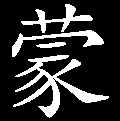
\includegraphics[width=3mm]{../Images/00006}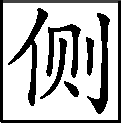
\includegraphics[width=3mm]{../Images/00011}\footnotesize \kaishu 老人家神影活现。}``先打死我,再打死他,岂不干净了!''贾政见他母亲来了,又急又痛,连忙迎接出来,只见贾母扶着丫头,喘吁吁的走来。

贾政上前躬身陪笑道:``大暑热天,母亲有何生气亲自走来?有话只该叫了儿子进去吩咐。''贾母听说,便止住步喘息一回,{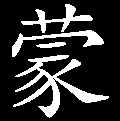
\includegraphics[width=3mm]{../Images/00006}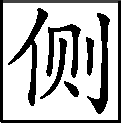
\includegraphics[width=3mm]{../Images/00011}\footnotesize \kaishu 大家规模,一丝不乱。}厉声说道:``你原来是和我说话!我倒有话吩咐,只是可怜我一生没养个好儿子,却教我和谁说去!''贾政听这话不像,忙跪下含泪说道:``为儿的教训儿子,也为的是光宗耀祖。母亲这话,我做儿的如何禁得起?''贾母听说,便啐了一口,说道:``我说一句话,你就禁不起,你那样下死手的板子,难道宝玉就禁得起了?{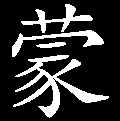
\includegraphics[width=3mm]{../Images/00006}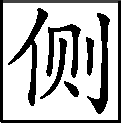
\includegraphics[width=3mm]{../Images/00011}\footnotesize \kaishu 偏有是理。}你说教训儿子是光宗耀祖,当初你父亲怎么教训你来!''{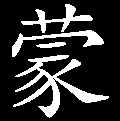
\includegraphics[width=3mm]{../Images/00006}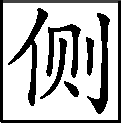
\includegraphics[width=3mm]{../Images/00011}\footnotesize \kaishu 如此碍犯文字,随景生情,毫无牵滞。}说着,不觉就滚下泪来。

贾政又陪笑道:``母亲也不必伤感,皆是作儿的一时性起,从此以后再不打他了。''贾母便冷笑道:``你也不必和我使性子赌气的。你的儿子,我也不该管你打不打。我猜着你也厌烦我们娘儿们。不如我们赶早儿离了你,大家干净!''说着便令人去看轿马,``我和你太太宝玉立刻回南京去!''家下人只得干答应着。贾母又叫王夫人道:``你也不必哭了。如今宝玉年纪小,你疼他,他将来长大成人,为官作宰的,也未必想着你是他母亲了。你如今倒不要疼他,只怕将来还少生一口气呢。''贾政听说,忙叩头哭道:``母亲如此说,贾政无立足之地。''贾母冷笑道:``你分明使我无立足之地,你反说起你来!只是我们回去了,你心里干净,看有谁来许你打。''一面说,一面只令快打点行李车轿回去。贾政苦苦叩求认罪。

贾母一面说话,一面又记挂宝玉,忙进来看时,只见今日这顿打不比往日,又是心疼,又是生气,也抱着哭个不了。王夫人与凤姐等解劝了一会,方渐渐的止住。早有丫鬟媳妇等上来,要搀宝玉,凤姐便骂道:{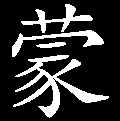
\includegraphics[width=3mm]{../Images/00006}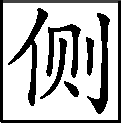
\includegraphics[width=3mm]{../Images/00011}\footnotesize \kaishu 能事者自不凡。}``糊涂东西,也不睁开眼瞧瞧!打的这么个样儿,还要搀着走!还不快进去把那藤屉子春凳抬出来呢。''众人听说连忙进去,果然抬出春凳来,将宝玉抬放凳上,随着贾母王夫人等进去,送至贾母房中。

彼时贾政见贾母气未全消,不敢自便,也跟了进去。看看宝玉,果然打重了。再看看王夫人,``儿''一声,``肉''一声,``你替珠儿早死了,留着珠儿,免你父亲生气,我也不白操这半世的心了。这会子你倘或有个好歹,丢下我,叫我靠那一个!''数落一场,又哭``不争气的儿''。贾政听了,也就灰心,{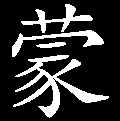
\includegraphics[width=3mm]{../Images/00006}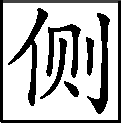
\includegraphics[width=3mm]{../Images/00011}\footnotesize \kaishu 天下作父兄者,教子弟时亦当留意。}自悔不该下毒手打到如此地步。先劝贾母,贾母含泪说道:``你不出去,还在这里做什么!难道于心不足,还要眼看着他死了才去不成!{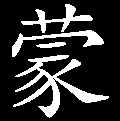
\includegraphics[width=3mm]{../Images/00006}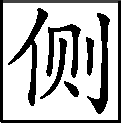
\includegraphics[width=3mm]{../Images/00011}\footnotesize \kaishu 遣之有法。}''贾政听说,方退了出来。

此时薛姨妈同宝钗、香菱、袭人、史湘云也都在这里。袭人满心委屈,只不好十分使出来,见众人围着,灌水的灌水,打扇的打扇,自己插不下手去,便越性走出来到二门前,令小厮们找了茗烟来细问:{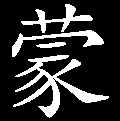
\includegraphics[width=3mm]{../Images/00006}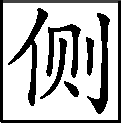
\includegraphics[width=3mm]{../Images/00011}\footnotesize \kaishu 各自有各自一番作用。}``方才好端端的,为什么打起来?你也不早来透个信儿!''茗烟急的说:``偏生我没在跟前,打到半中间我才听见了。忙打听原故,却是为琪官金钏姐姐的事。''袭人道:``老爷怎么得知道的?''茗烟道:``那琪官的事,多半是薛大爷素日吃醋,没法儿出气,不知在外头唆挑了谁来,在老爷跟前下的火。那金钏儿的事是三爷说的,我也是听见老爷的人说的。''袭人听了这两件事都对景,心中也就信了八九分。然后回来,只见众人都替宝玉疗治。调停完备,贾母令``好生抬到他房内去''。众人答应,七手八脚,忙把宝玉送入怡红院内自己床上卧好。又乱了半日,众人渐渐散去,袭人方进前来经心扶侍,问他端的。且听下回分解。

{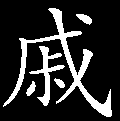
\includegraphics[width=3mm]{../Images/00005}总评:严酷其刑以教子,不情中十分用情;牵连不断以思婢,有恩处一等无恩。严父慈母一般爱子,亲优溺婢总是乖淫。蒙头花柳,谁解春光?跳出樊笼,一场笑话!}

{\href{../Text/part0037_split_000.html\#navto_1_a}{①}长史官这段话,列藏本有独特异文:``\ldots{}\ldots{}我们府里有一个作小旦的琪官,那原是奉旨由内园赐出,只从出来,好好在府里住了不上半年,如今三日五日不见了,各处去找,又摸不着他的道路,因此各处察访。这一城内,十停人到有八停人都说,他竟日和衔玉的那位令郎相与甚厚。下官辈听了,尊府不比别家,可以擅来索取,因此启明王爷。王爷亦云:`若是别的戏子,一百个也罢了,只是这琪官,乃奉旨所赐,不便转赠令郎。'若令郎十分爱慕,老大人竟密题一本请旨,岂不两便。若大人不题奏时,还得转达令郎,请将琪官放出。一则可免王爷负恩之罪,二则下官辈也可免操劳求觅之苦。''比别本多出的话,是拉扯上朝廷,称琪官乃``奉旨所赐'',如此上纲上线,宝玉的罪名就大了。这段异文究竟是作者原稿,还是后人妄改,学界存在不同看法,录以备考。}

{\href{../Text/part0037_split_000.html\#navto_2_a}{②}``兴来'',除列本作``来兴儿来''、杨本作``来兴''外,诸本均同。按``兴来''不通,故诸校本多据杨、列本校改作``来兴'',这样就衍生了一个人名出来。虽然书中偶有这种昙花一现的人物,但此处贾政要找管理家务的人来问话,一个主子贾琏、一个奴才大总管赖大,已经够了,也无须第三人的。目前没有其他更好的校法,暂参程本删``兴''字。}
